%% 
%% Created in 2018 by Martin Slapak
%%
%% Based on file for NRP report LaTeX class by Vit Zyka (2008)
%%
%% Compilation:
%% >pdflatex report
%% >bibtex report
%% >pdflatex report
%% >pdflatex report

\documentclass[czech]{mvi-report}

\usepackage[utf8]{inputenc} 

\title{Generování obrázků maleb z fotografií}

\author{Luboš Zápotočný}
\affiliation{ČVUT - FIT}
\email{zapotlub@fit.cvut.cz}

\def\file#1{{\tt#1}}

\begin{document}

\maketitle

%%%%%%%%%%%%%%%%%%%%%%%%%%%%%%%%%%%%%%%%%%%%%%%%%%%%%%%%%%%%%%%%%%%%%%%%%%%%%%%%
\section{Úvod}
GAN se skládá ze dvou neuronových sítí: model generátoru a model diskriminátoru.

Generátor je (hluboká) neuronová síť, která vytváří obrázky. Pro daný dataset se snažím generovat obrázky ve stylu malíře Moneta. Tento generátor je trénován pomocí diskriminátoru.

Tyto dva modely pracují proti sobě, přičemž generátor se snaží oklamat diskriminátor a diskriminátor se snaží přesně klasifikovat skutečné vs. generované obrázky.

Cílem je vybudovat GAN, který generuje 7000 obrázků ve stylu malíře Moneta z reálných fotografií.

Transformaci z reálné fotografie na obrázek, který se bude co nejvíce podobat malířskému stylu použiji jeden z modelů pro tzv. style transfer, konkrétně CycleGAN.

Transformace obrázku na obrázek je problém, kde je cílem naučit se mapování mezi vstupním obrázkem a výstupním obrázkem pomocí trénovací sady zarovnaných párů obrázků. Zarovnané obrázky jsou takové, u kterých máme k dispozici zdrojový obrázek a také příslušný obrázek po transformaci. Bohužel takovýto dataset není vždy možné vytvořit. Například při transformaci zimní krajiny na letní bychom museli vyfotit mnoho míst v zimním období a na úplně stejném místě za 6 měsíců vytvořit ideálně úplně stejnou fotku. U jiných příkladů již takové mapování ani není možné vytvořit. Například u obrazů, které namalovali malíři před stovkami let se ani neví, kde dané namalované místo může být.

Tvorba datasetu je tedy buď časově nebo peněžně velmi nákladná a v některých případech i nemožná. CycleGAN umožňuje vytrénovat model hlubokého učení, který se dokáže tuto transformaci naučit i bez zarovnaných (spárovaných) dat. \cite{GAN}, \cite{CycleGAN}, \cite{mosquera_2020}, \cite{kikaben_2022}, \cite{brownlee_2020_cyclegan}, \cite{brownlee_2020_conv}, \cite{brownlee_2019_batch}, \cite{brownlee_2019_norm}

%%%%%%%%%%%%%%%%%%%%%%%%%%%%%%%%%%%%%%%%%%%%%%%%%%%%%%%%%%%%%%%%%%%%%%%%%%%%%%%%
\section{Vstupní data}

Vstupní data jsem převzal ze soutěžního datasetu na webové stránce Kaggle.com

Dataset obsahuje 300 obrázků (256x256 pixelů) některých částí obrazů od malíře Moneta. A obsahují více než 7000 fotografií různého druhu u kterých se očekává převedení stylu malby Moneta na tyto fotografie.

Ukázka datasetu je vyobrazena na obrázku \ref{fig:input-data}.

\begin{figure}[h]
  \centering\leavevmode
  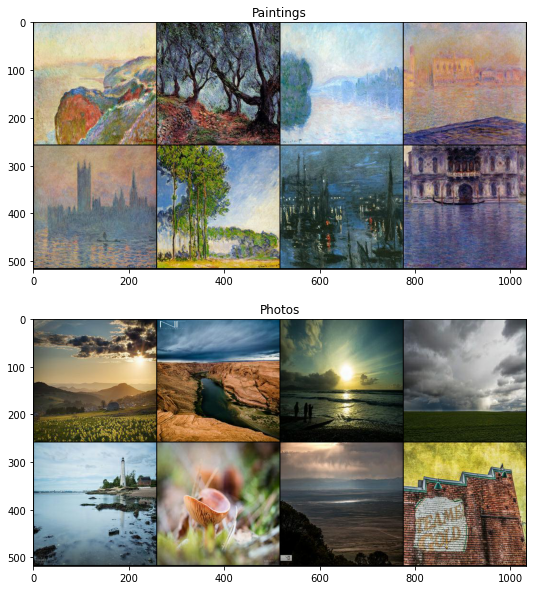
\includegraphics[width=1\linewidth]{img/paintings_photos}\vskip-0.5cm
  \caption{Ukázka vstupních dat}
  \label{fig:input-data}
\end{figure}

%%%%%%%%%%%%%%%%%%%%%%%%%%%%%%%%%%%%%%%%%%%%%%%%%%%%%%%%%%%%%%%%%%%%%%%%%%%%%%%%
\section{Metody}

Jako první bych chtěl zmínit, že bylo nutné přibližně skoro 10 hodin řešit výkon nahrávání obrázků z Google disku, který byl připojen do běhového prostředí Google Colab. Takto vytvořené sítové připojení disku mělo velmi negativní dopad na rychlost načítaní dávek (batches) při nahrávání dat pro trénování modelů.

Tento problém byl vyřešen efektivní archivačním algoritmem, který mi dovolil vstupní data (obrázky) uložit na vzdálené úložiště (github repozitář, archiv má < 100MB) a při inicializaci trénovacího Notebooku data stáhnout, extrahovat a používat jako lokální složku v běhovém prostředí. Efektivita čtení obrázků (z disku) se násobně zrychlila.

Výzkum CycleGAN zmiňuje použití ResNET architektury, kterou budu chtít porovnat s UNet architekturou.

%%%%%%%%%%%%%%%%%%%%%%%%%%%%%%%%%%%%%%%%%%%%%%%%%%%%%%%%%%%%%%%%%%%%%%%%%%%%%%%%
% --- VYSLEDKY
\section{Výsledky}

Výsledný style transfer není dokončený. Chybí implementovat trénovací část a díky experimentálnímu vyhodnocení ladit parametry modelů a případně struktury jednotlivých komponent. 

Prozatím jsem se soustředil na detailní rešerši o obsáhlých tématech. Zároveň jsem se snažil pochytit best-practices s prací s PyTorch.

Obrázek \ref{fig:test-generator} vyobrazuje první spuštění generátoru na vstupních datech. Zatím není aplikované učení pomocí diskriminátoru, ale i tak je vidět, že konvulenční vrstva zafungovala. 

\begin{figure}[h]
  \centering\leavevmode
  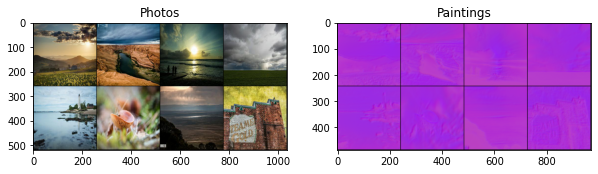
\includegraphics[width=1\linewidth]{img/first_result_wip}\vskip-0.5cm
  \caption{Testování generátoru (bez trénování)}
  \label{fig:test-generator}
\end{figure}

%%%%%%%%%%%%%%%%%%%%%%%%%%%%%%%%%%%%%%%%%%%%%%%%%%%%%%%%%%%%%%%%%%%%%%%%%%%%%%%%
% --- ZAVER
\section{Závěr}

Základní struktura trénovacích komponent byla vytvořena a byl vyřešen problém pomalého načítání z Google disku na běhovém prostředí Google Colab.

Práce prozatím není dokončená a chybí jí trénovací fáze modelu. Každopádně základní komponenty generátorů a diskriminátorů jsou již v první verzi připravené a budou v následujících iteracích vylepšovány tak, aby obsahovali co nejvíce poznatků z výzkumu CycleGAN a dosahovaly uspokojivých výsledků.

Rád bych tuto práci využil jako reprezentativní práci v nadcházejících projektech a chtěl bych vytrénovaný model vyzkoušet na real-time převodu videa. 

%%%%%%%%%%%%%%%%%%%%%%%%%%%%%%%%%%%%%%%%%%%%%%%%%%%%%%%%%%%%%%%%%%%%%%%%%%%%%%%%
% --- Bibliography

%\bibliographystyle{plain-cz-online}
\bibliography{reference}

\end{document}
